% !TEX root = /home/fred-olav/afgv/src/preamble.tex
% Start preamble
\documentclass[10pt,a5paper,norsk]{article}
\usepackage{geometry}
 \geometry{
 a5paper,
 total={120mm,185mm},
 left=10mm,
 top=10mm,
 }
\usepackage[utf8]{inputenc}
\usepackage[table]{xcolor}
\usepackage[T1]{fontenc}
\usepackage[pdftex]{graphicx}
\graphicspath{{./}}
\usepackage{enumitem}
\usepackage{pdfpages}
\usepackage{hyperref}
\usepackage{tikz}
\usepackage{attachfile}
\usepackage[ngerman]{babel}
\usepackage{epstopdf}
\usepackage{array}
\usepackage{longtable}
%\usepackage[table,xcdraw]{xcolor}
\usepackage{amsmath}
\usepackage{makecell}
\usepackage{multirow}
%\setlength{\textwidth}{11cm}
%\setlength{\oddsidemargin}{-0.5cm}
\setlength{\evensidemargin}{-1.5cm}
%\setlenght{\headsep}{0cm}
\setlength\parindent{0pt}
%\setlength{\extrarowheight}{3pt}
\usepackage{listings}
\usepackage{microtype}
\usepackage{setspace}
\usepackage{verbatim}
\usepackage{wrapfig}
%\usepackage{xcolor}

\input{../src/arduinoLanguage.tex}

\include{def}
% End preamble

\begin{document}
\huge
\begin{center}
\textbf{Håndbok for 3AUA Gand VGS} \bigskip
\end{center}

\vskip 1cm
		$$\includegraphics[height=15cm]{../output/nogpl/elektro_tr.png}$$
\normalsize
\vfil \eject

\section {Utførelse av arbeidsoppdrag}
%Måleteknikk 
\hrule

\vskip 1cm

I 3AUA utføres praktisk arbeid som arbeidsoppdrag, disse skal bestå av følgende:\begin{itemize}[noitemsep]
	\item Planlegging
	\item Gjennomføring
	\item Dokumentasjon
\end{itemize}

\subsection {Planlegging}

Planleggingen av arbeidsoppdragene har som hensikt å:

\begin{itemize}[noitemsep]
	\item Sørge for at vi har kunnskap nok til å starte opp arbeidet. 
	\item Tenke igjennom hva arbeidet består av og i hvilken rekkefølge det er hensiktmessig å utføre det. 
	\item Sørge for av vi har alt nøvendig utstyr og materiell. 
\end{itemize}



Alt arbeid skal risikovurderes før utførelse. Nødvendig sikringstiltak skal planlegges og utføres i henhold til bedriftens HMS-regelverk. Eksempelvis skal all energitilførsel stenges og sikres mot utilsiktet innkopling, hvis mulig. Hvis ikke, skal arbeidene planlegges og utføres under gjeldende sikringstiltak, eksempelvis med AUS verktøy isolerende matter, etc. Husk spesielt personlig verneutstyr, så som briller, hjelm, hansker, sko, klær, hørselvern, etc.

Planleggingsdlen skal innholde:

\textbf{Innledning:}
\vskip 10pt 
\vskip 10pt 
\textbf{Fremdriftsplan:}
\vskip 10pt 
Skal vise at du forstår hva som inngår av arbeid i de ulike oppdragene og at du forstår i hvilken rekkefølge de må utføres. Denne er også et greit utgangpunkt for å hvilke deler som sakl være med i en risikovurdering. 


\vskip 10pt 
SJA skal utføres om et arbeid ikke er kjent eller det finnes rutine for det. Som elev i et fag vil det si at i de flese arbeidsoppdrag må det utføres en SJA. 
\vskip 10pt 
\textbf{Verktøysliste:}
\vskip 10pt 
Skal vise at du vet hvilket verktøy som trengs til de ulike jobbene. Å bruke korrekt navn er en viktig del. 

\vskip 10pt 
\textbf{Utstyrsliste:}
\vskip 10pt 
Skal vise at du vet hvilket utstyr som trengs til de ulike jobbene. Å bruke korrekt navn er en viktig del. Utstyrslisten skal inneholde det som du ville tatt betalt for av en kunde. 

\vskip 10pt 
\textbf{HMS Risikovurdering:}
\vskip 10pt 
Skal vise at du kan vurdere farer med arbeidet og sette inn tiltakt for å unngå farene. FSE er sentral i forhold til farer med elektrisitet. 

\vskip 5pt 
\vskip 10pt 
\textbf{Teori, Instrumenter og utstyr:}
\vskip 10pt 
\vskip 5pt 
Her legger du inn forklaring for virkemåte og rolle i anlegget for valgte instrumenter og utstyr. Du forklarer også sentral teori for anlegget.

\vskip 5pt 
\textbf{Koblingstegninger:}

Her legger du ved skjema for alle oppkoblinger du planlegger. 

\vskip 10pt 
\vskip 10pt 
\textbf{Lover, forskrifter og normer:}
\vskip 10pt 
Her beskriver du hvilke lover, forskrifter og normer som er relevante for arbeidet. 
\subsection{Gjennomføring}

Enten arbeidsoppdraget skal utføres i praksis eller det bare er en del av en prøve skal gjennomføringenen beskrives. Dette er viktig del øvelsen til å besvare eksamensoppgaver. 
\vskip 5pt 
Om du har utført arbeidet kan det være lurt å beskrive hvordan du ville utført arbeidet om du skulle gjort det en gang til. 
\subsection{Dokumentasjon}

\vskip 5pt 
Alle arbeidsoppdrag skal inneholde relevant dokumentajson i forhold til arbeidet som er gjort. Det kan f.eks. være et prosjekt der du må levere komplett dokumentajson. Et annet eksempel kan være kalibrering av en transmitter der en kort arbeidsrapport og et kalibreringsskjema vil være relevant. 

\subsection{Oversikt over arbeidsoppdrag}
\begin{center}
	\begin{tabular}{| m{2cm} |m{2cm} |m{5cm} |m{1cm} |} 
\hline
	\multicolumn{4}{|c|}{\textbf{\cellcolor[HTML]{D5D5D5}Oversikt over arbeidsoppdrag}} \\
\hline
\hline
\rowcolor [HTML]{D5D5D5}
Fil	&Stasjon&Emne&Utført\\ \hline
	i04820.tex  & Stasjon 01 & Gandsfjorden Gondol& \\ \cline{1-4}
	i04823.tex  & Stasjon 02 & IO-sjekk&\\ \cline{1-4}
	i04834.tex  & Stasjon 02 &  Profinet tutorial&\\ \cline{1-4}
	lStasjon03.tex  & Stasjon3/4/5 & Oppsett av reguleringsstasjon&\\ \cline{1-4}
	i04862.tex  & Stasjon 06 & Vision med robot &\\ \hline
	lStasjon09.tex  & Stasjon 09 & Målesystemer for nivå&\\ \cline{1-4}
	i04842.tex  & Stasjon 10 & Målesystemer for trykk&\\ \cline{1-4}
	i04841.tex  & Stasjon 11 & Målesystemer for temperatur& \\ \cline{1-4}
	i04831.tex  & Stasjon 12 & HMI til byggautomasjon & \\ \cline{1-4}
	lStasjon13.tex  & Stasjon 13 & Reguleringsmodell for strømning&\\ \cline{1-4}
	lStasjon14.tex  & Stasjon 14 & Sjekk av kommnkikasjonsnett&\\ \cline{1-4}
	lStasjon15.tex  & Stasjon 15? & Digitale målesystemer &\\ \hline
	i04821.tex  & Stasjon 16 & Sikkerhetsrele& \\ \cline{1-4}
	i04825.tex  & Stasjon 16 & Sikkerhets PLS &\\ \cline{1-4}
	i04858.tex  & Stasjon 20 & Servo med motion control bolokker&\\  \cline{1-4}
\end{tabular}
\end{center}


\section{Rutiner}

Rutiner beskriver hvordan den daglige oppførselen skal være. 

\subsection{Rydding}

\subsubsection{Personlige eiendeler}
\begin{enumerate}
\item Yttertøy henges på knagger
\item Arbeidsklær skal henge i skapet 
\item Verktøykasse skal stå under benk bak i klasserommet.
\item Bøker som ikke brukes i timen skal være innelåst i skap. 
\end{enumerate}

\vfil \eject

\section{Dokumentasjon}
\subsection{P \& ID} 

Vi tegner P \& ID etter ISO 15519-2 Standaren. Det brukes mange standrer
for P\&ID, men denne er ny og oppdatert. Når en møter på eldre standarder
må en tolke så godt en kan og kanskje finne en beskrivelse i en gammel
norm o.l...

ISO 15519 henter symboler fra ISO 14617 serien. 

ISO 15519-1:2010 Specification for diagrams for process industry \textemdash{}
Part 1: General rules

ISO 15519-2:2015 Specifications for diagrams for process industry
\textemdash{} Part 2: Measurement and control

Kjemisk industri og petroliumsindustien har sin egen standard, som
bygger på ISO 15519, ISO 10628-1 (Diagrams for the chemical and petrochemical
industry. 
Frem til nå har vi sett på flere typer instrument skjema, i alle har de for skjellige instrumentene hatt en kode som forklarer funksjonen. TT er en Termperatur Transmitter, PDT er en Trykk Differanse Transmitter eller FV er en Flow Ventil. Disse bokstavene er definert i ISO 14617-6. 

\vskip 5pt 

\vskip 5pt 

\vskip 5pt 


\vskip 5pt 

% No blank lines allowed between lines of an \halign structure!
% I use comments (%) instead, so that TeX doesn't choke.
\hrule
\small
\begin{center}
\begin{tabular}{ | m{1cm} | m{2.5cm}| m{2cm} | m{2.5cm} |} 
\hline
\multicolumn{4}{|c|}{Bokstavkode for indentifisering av instrumentfunksjoner} \\
\hline
	Bokst. & Variabel& Omformer & Funksjon \\ 
\hline
	A&&&Alarm\\
\hline
	B&&&Visning av diskre status\\
\hline
	C&&&Regulerende\\
\hline
	D&Densitet&Differanse&\\
\hline
	E&Elektrisk variabel&&Elemens (følende)\\
\hline
	F&Flow rate&Forhold&\\
\hline
	G&Posisjon, lengde&&Visning\\
\hline
	H&Håndbetjent&&\\
	\hline
	I&&&Indikerende\\
	\hline
	J&Effekt&Avsøke&\\
	\hline
	K&Tid&Forandring i tid&\\
	\hline
	L&Nivå&&\\
	\hline
	M&Fuktighet eller Relativ fuktighet&&\\
	\hline
	N&Etter brukers valg&&\\
	\hline
	N&Etter brukers valg&&\\
	\hline
	P&Trykk eller vakum&&Tilkobling til testpunkt\\
	\hline
	Q&\makecell{Egenskap\\f.eks:\\*Analyse\\*Konsentrasjon}&Integrere eller summere&Integrerende eller summerende\\
	\hline
	R&Radioaktiv stråling&&Skrivende\\
	\hline
	S&Hastighet&&Bryterfunksjon\\
	\hline
	T&Temperatur&&Overføring\\
	\hline
	U&Multivariabel&&Multifunksjon\\
	\hline
	V&Etter brukers valg& &Påvirkning på prosess med ventil eller pumpe, o.l.\\
	\hline
	W&Vekt, Kraft&Multipliserende&\\
	\hline
	X&Uspesifiserte variabler&&Uspesifisert\\
	\hline
	Y&Etter brukers valg&&Konvertering eller algoritme\\
	\hline
	Z&Antall hendelser, antall&&Nødbetjening eller sikkerhetsfunksjon\\
\hline
\end{tabular}
\end{center}
\normalsize
%Måleteknikk 
\vskip 5pt
\hrule

\vskip 5pt

\subsection{Tegneregler}

\subsubsection{Linjetykkelser}
\begin{itemize}
\item 1.0 mm skal brukes for hovedprosesslinjer
\item 0.5 mm skal brukes på:
\begin{itemize}
\item symboler som representerer makineri, unntatt ventiler og fittings
\item rektangulære rammer som representerer enhetsoperasoner, prosessutstyr,
o.l.
\item Tilleggs prosesslinjer
\item energiforsyningslinjer.
\end{itemize}
\item 0.25 mm skal brukes på.
\begin{itemize}
\item symboler som representerer ventiler, fitting og rørtilbehør.
\end{itemize}
\end{itemize}

\subsection{Informasjonsflyt mellom kontrollsystemet og prosessen. }

\includegraphics[width=1\textwidth]{./PandID01.eps}

\subsection{Plassering av informasjon rundt PCI symboler. }

%\includegraphics[width=0.5\textwidth]{P&ID04}
\subsubsection{Inn og ut av skjemaer}

Linjer som skal fortsette i andre skjemaer skal ha en PIL

%\includegraphics{P&ID05}

Pil for inn- og utgående flow

%\includegraphics{P&ID06}


\subsection{Referansebetegnelsessystem}
\small
\begin{center}
\begin{tabular}{ | m{1cm} | m{2.5cm}| m{2cm} | m{2.5cm} |} 
\hline
\multicolumn{4}{|c|}{Bokstavkode for utstyri} \\
\hline
	Bokst. & Variabel& Omformer & Funksjon \\ 
\hline
	A&&&Alarm\\
\hline
	B&Sensorer&&Visning av diskre status\\
\hline
	C&Lagring&&Regulerende\\
\hline
	E&Strålende objekt&&\\
\hline
	F&Beskyttende objekt&&\\
\hline
	G&Beskyttende objekt&&\\
\hline
	H&Prossesring av materie&&\\
	\hline
	K&Prosessring av informasjon&&\\
	\hline
	L&Nivå&&\\
	\hline
	M&Objekt som driver noe&&\\
	\hline
	N&&&\\
	\hline
	P&objekt som presenterer&&\\
	\hline
	Q&objekt som presenterer&&\\
	\hline
	R&Objekt som begrenser&&\\
	\hline
	S&Objekt for betjening &&\\
	\hline
	T&Transformerende objekt&&\\
	\hline
	U&Objekt som holder&&\\
	\hline
	W&Førende objekt&&\\
	\hline
	X&Objekt for overgang&&\\
	\hline
\hline
\end{tabular}
\end{center}
\normalsize
%Måleteknikk 
\vfil \eject
\subsection{Symboler}
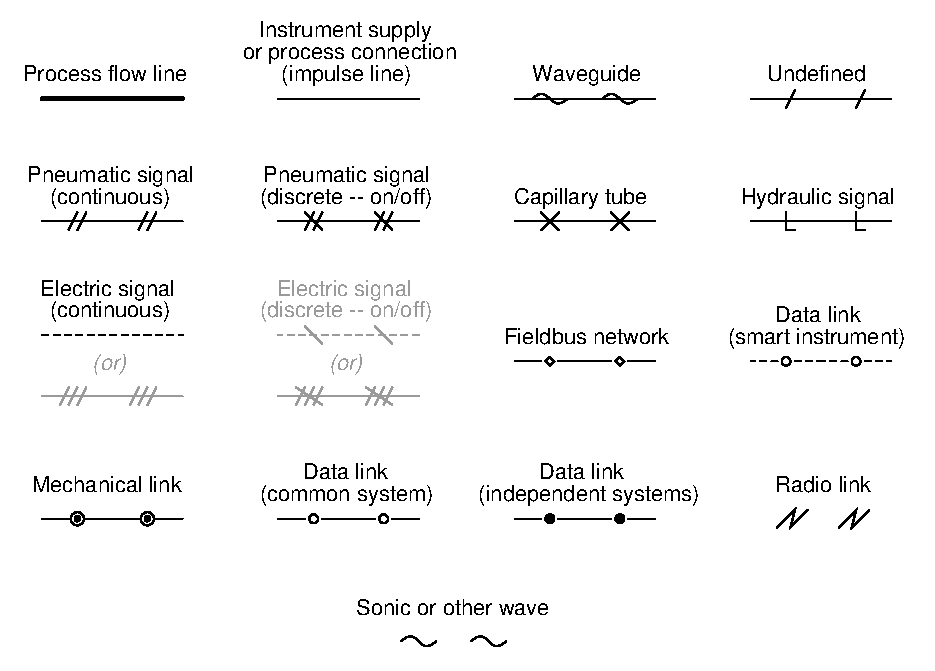
\includegraphics[width=1\textwidth]{diagrams00.eps}
\includegraphics[width=1\textwidth]{diagrams01.eps}
\includegraphics[width=1\textwidth]{diagrams03.eps}
\includegraphics[width=1\textwidth]{diagrams13.eps}
\includegraphics[width=1\textwidth]{diagrams05.eps}
\includegraphics[width=1\textwidth]{diagrams02.eps}
%\includegraphics[width=1\textwidth]{diagrams04.eps}
%\includegraphics[width=1\textwidth]{diagrams06.eps}
%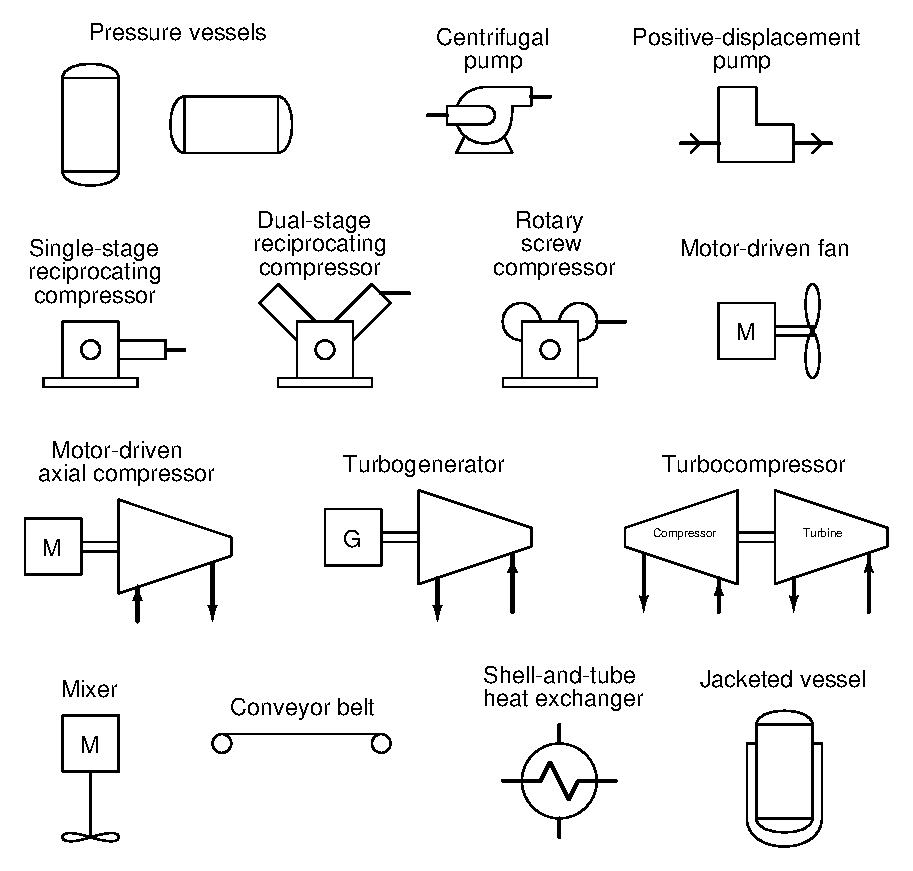
\includegraphics[width=1\textwidth]{diagrams07.eps}
%\includegraphics[width=1\textwidth]{diagrams10.eps}
%\includegraphics[width=1\textwidth]{diagrams11.eps}
%\includegraphics[width=1\textwidth]{diagrams12.eps}
%\includegraphics[width=1\textwidth]{diagrams14.eps}
\newpage


\section{Instrumentering}
%Måleteknikk

\begin{center}
\begin{longtable}{ | m{2cm} | m{7cm} | } 
\hline
\multicolumn{2}{|c|}{Definisjoner} \\
\hline
Begrep	& Beskrivelse \\ 
\hline
\hline
	Avvik&Forskjellen mellom den målte verdien og ønsket verdi (skalverdi) i ei reguleringssløyfe\\
	\hline
	Dødgang (dødsone)&For prosessinstrumenter er dødgang det området som et inngangssignal kanforandres innenfor, uten at det vises noen forandring i utgangssignalet. Med forandring menes her reversering av retningen på inngangssignalet\\
	\hline
	Forsterkning&Forholdet mellom forandring i inngangsverdien i forhold til den utgangsverdien som var årsak til forandringen\\
	\hline
	Hysterese&Samme måleverdi kan gi ulike utsignaler fra måleomformeren ved samme verdi, Hysterese oppstår når måleverdien veksler mellom å være stigende eller fallende.\\
	\hline
	Kalibrering&Sjekk av at måleinstrumentets verdier stemmer med et intrument med høyere nøyaktihet. Noen intrumenter kan justeres inn om de ikke stemmer overens.\\ 
	\hline
	Lesbarhet&Den minste inndeling på skalaen på et instrument.\\
	\hline
	Måleomfang&Differansen mellom øvre og nedre målegrense\\
	\hline
	Målegrense&URV: høyeste verdi som instrumentet kan vise. LRV: laveste verdi som instrumentet kan vise. \\
	\hline
	Målegrense&Den fulle skalaen for en måling, indikering eller avlesning. Eksempelvis -50 til 150°C\\
	\hline
	Nullpunktfeil&En forskyving av nede målegrense\\
	\hline
	Nøyaktighet& Forskjell mellom avlest og virkelig verdi for en målt variabel.\\
	\hline

	Reproduser- barhet& Evnen til å reprodusere samme resultat fra en rekke uavhengige målinger av den samme verdien selv om målingen utføres av forskjellige personer, på forskjellige steder og under ulike klimatiske forhold.\\
	\hline
	Repeterbarhet&Samsvar mellom en rekke på hverandre følgende målinger av utgangsverdi for den samme inngangsverdien. Målingene foretas under samme klimatiske forhold, av samme person og med korte intervaller.\\
	\hline
	Ulinearitet&En type feil der inngangsverdiene til et instrument ikke forholder seg til den ideelle rettlinjede sammenhengen mellom inngangs- og utgangs-verdiene (referansekarakteristikken).\\
	\hline

Regulator & En enhet som har til oppgave å påvirke prosessen slik at den oppnår en ønsket tilstand (f.eks. et ønsket nivå eller en ønsket temperatur).\\
	\hline
Prosess & Det anlegget eller systemet som inngår i reguleringen.\\
	\hline
Prosessvariabel & Den fysiske størrelsen i prosessen som skal reguleres (nivå, trykk, temperatur etc.)\\
	\hline
ProsessVerdi PV & Den verdien prosessvariabelen til enhver tid har.\\
	\hline
Settpunkt SP & Den verdien vi ønsker at prosessvariabelen skal ha.\\
	\hline
Manipulerende Variabel MV & Signalet som styrer pådragsorganet\\
	\hline
Forsyning & \\
	\hline
Pådrag & Det som er ment å variere prosessvariabelen. F.eks. væske inn i en nivåtank. \\
	\hline
Belastning & Det som tas ut av prosessen ved konstant PV. Vil ha samme verdi som pådraget. \\
	\hline
Forstyrrelse & Forandringer som påvirker verdien til prosessvariabelen. \\
	\hline
Avviket e & Forskjellen mellom PV og SP (Direkte virkning PV-SP, Reverserende virkning SP-PV)\\
	\hline
Pådragsorgan & Den komponenten som styrer pådraget (f.eks. motoren i bilen som påvirker hastigheten, eller ventilen som påvirker nivået i tanken).\\
	\hline
Forstillingsenhet & I vårt eksempel med regulering av bilens hastighet, er forstillingsenheten forgasseren. Motoren er pådragsorganet i reguleringssløyfen.\\
	\hline
Auto og Manuell modus (Lukket& eller åpensløyfe). Om pådraget styres av regulatoren eller en manuell innstilt verdi. \\
	\hline
LRV og URV& ( Lover Range Value og Upper Range value, Laveste og høyeste verdi målesignalet kan ha.)\\

	\hline


\end{longtable}
\end{center}
\vskip 5pt
\hrule

\vskip 5pt
\subsection{Kalibrering}
Kalibrering vil si at en sjekker at måleinstrumentets verdier stemmer med et intrument med høyere nøyaktihet. Noen intrumenter kan justeres inn om verdien ikke er innenfor kravet. Etter denne justeringen kan en da gjøre en ny sjekk av måleinstrumentets verdier. 

\vskip 5pt 
$$\includegraphics[width=1\textwidth]{calibrate31.eps}$$

\filbreak

$$\includegraphics[width=1\textwidth]{calibrate26.eps}$$
$$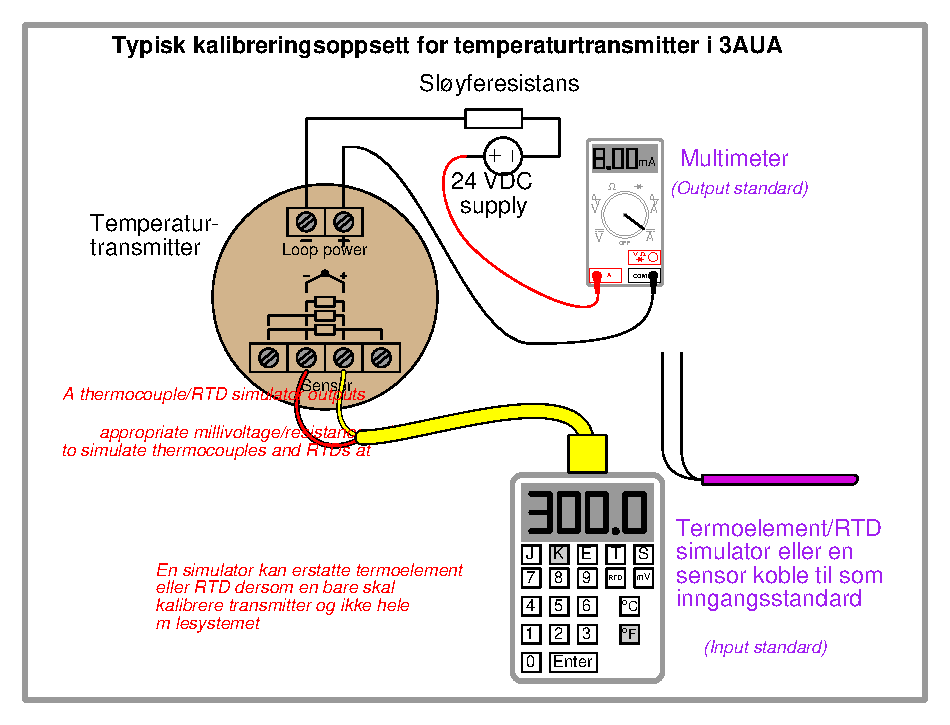
\includegraphics[width=1\textwidth]{calibrate32.eps}$$
\filbreak
\vskip 5pt 

I 3AUA bruker vi 5-punkts opp/ned sjekk når vi kalibrerer instrumenter. 

\vfil \eject
\large
\begin{center}
\begin{tabular}{ | m{2cm} | m{2cm} |m{2cm} |m{2cm} |m{2cm} |} 
\hline
	\multicolumn{5}{|c|}{\textbf{\cellcolor[HTML]{D5D5D5}Kalibreringsskjema for 3AUA Gand}} \\
\hline
\hline
\hline
	\multicolumn{5}{|c|}{\textbf{\cellcolor[HTML]{D5D5D5}Instrument informasjon}}\\
\hline
	System tag&	\multicolumn{2}{l|}{Produsent}&\multicolumn{2}{l|}{Modell}\\
\hline
&	\multicolumn{2}{l|}{}&\multicolumn{2}{l|}{}\\
\hline
	C.Intervall&\multicolumn{2}{l|}{Serienr.}&LRV&URV\\
\hline
	&	\multicolumn{2}{l|}{}&&\\
\hline
	\multicolumn{5}{|c|}{\textbf{\cellcolor[HTML]{D5D5D5}Feil \%} }\\
\hline
	Største feil&Zero&Span&Liearitet&Hysterese\\
\hline
	&&&&\\
\hline
	\multicolumn{5}{|c|}{\cellcolor[HTML]{D5D5D5}\textbf{As Found resultater}}\\
\hline
	Test punkt	&Inngang&Utgang&Utgangsfeil&Utg.feil \%\\
\hline
1&&&&\\
\hline
2&&&&\\
\hline
3&&&&\\
\hline
4&&&&\\
\hline
5&&&&\\
\hline
4&&&&\\
\hline
3&&&&\\
\hline
2&&&&\\
\hline
1&&&&\\
\hline
	\multicolumn{5}{|c|}{\cellcolor[HTML]{D5D5D5}\textbf{As left resultater}}\\
\hline
	Test punkt	&Inngang&Utgang&Utgangsfeil&Utg.feil \%\\
\hline
1&&&&\\
\hline
2&&&&\\
\hline
3&&&&\\
\hline
4&&&&\\
\hline
5&&&&\\
\hline
4&&&&\\
\hline
3&&&&\\
\hline
2&&&&\\
\hline
1&&&&\\
\hline
	\multicolumn{5}{|c|}{\textbf{\cellcolor[HTML]{D5D5D5}Underskrifter}}\\
\hline
	\multicolumn{5}{|l|}{\textbf{Dato:}}\\
\hline
	\multicolumn{3}{|l|}{\textbf{Elev}}&\multicolumn{2}{l|}{\textbf{Lærer}}\\
\hline
	\multicolumn{3}{|c|}{}&\multicolumn{2}{c|}{}\\
\hline
\end{tabular}
\end{center}
\normalsize
\vfil \eject

\subsubsection{Generell sløyfetestprosedyre}
\begin{enumerate}
\item Sjekk at P\&ID tegning for denne sløyfa stemmer med Virkeligheten.
\item Oppdater P\&ID, evt. merk med \textquotedblright AS BUILT\textquotedblright ,
navn og dato
\item Sjekk at looptegningen for denne sløyfa stemmer med virkeligheten.
\item Oppdater looptegning, evt. merk med \textquotedblright AS BUILT\textquotedblright \textquotedblright ,
navn og dato.
\item Sjekk at datasheet for instrumentene i sløyfa stemmer.
\item Sjekk installasjon, (fyll ut \textquotedblright Punchlist\textquotedblright{}
for feil og mangler.)
\item Koble til HART communikator, sjekk at TAG nummer er lagt inn, sjekk
at LRV og URV stemmer med datasheet.
\item Sjekk at det er kalibreringssertifikat for alle instrumentene i sløyfa,
hvis ikke må instrumentene kalibreres og kalibreringssertifikat fylles
ut.
\item Simulering/testing
\begin{enumerate}
\item Ved simulering av trykk, sørg for å drenere/blåse ut evt. væske fra
transmitteren. Koble simulator for inngangssignal til transmitteren
(händpumpe/manometer) og mA meter på utgangen. Kjør 5 pkt. sjekk,
les av og noter resultat på alle instrumentene i sløyfa (kan kombineres
med pkt. 8) Ved tilbakekobling sørg for å lufte transmitteren, særlig
ved lave trykk.
\item Ved simulering av temperatur, koble simulator for inngangssignal til
transmitteren. (temperaturkalibrator eller dekadeboks etc. og mA meter
på utgangen. Kjør Spkt. sjekk, les av og noter resultat på alle instrumentene
i sløyfa (kan kombineres med pkt. 8). Koble tilbake elementet og sjekk
at transmitteren viser romtemperatur.
\end{enumerate}
\item Sjekk alarmsetpunkter og funksjon.
\item Fyll ut looptestsertifikat
\end{enumerate}





\vfil \eject
\subsubsection{skallering}
$$\includegraphics{current63.eps}$$

Ut fra denne representasjonen kan vi sette opp følgende formel for konvertering mellom signaler. 
$$		\frac{y-y_{start}}{y_{range}}=\frac{x-x_{start}}{x_{range}}$$

$$\includegraphics{current59.eps}$$
\vfil \eject


\section{HMI}

\subsubsection{Farger}
\begin{center}
\begin{tabular}{ | m{2.2cm} | m{2cm} |m{1.8cm} |m{5cm} |} 
\hline
	\multicolumn{4}{|c|}{\textbf{\cellcolor[HTML]{D5D5D5}Bruk av farger i HMI bilder for 3AUA Gand}} \\
\hline
	Fagre	&RGB verdi&Eksempel&Bruk\\
\hline
	Grå &213,213,213&{\cellcolor[HTML]{D5D5D5}}&Vanilg bakgrunn\\
\hline
	Hvit &255,255,255&{\cellcolor[HTML]{FFFFFF}}&Fremhevering av små\\
\hline
	Lys Grå &243,243,243&{\cellcolor[HTML]{F3F3F3}}&På indikasjon for utstyr\\
\hline
	Mørk Grå &74,74,74&{\cellcolor[HTML]{4A4A4A}}&Av indikasjon for utstyr\\
\hline
	Svart &0,0,0&{\cellcolor[HTML]{000000}}&\tiny Tekst, prosesslinjer og av grensing av prosessutstyr\normalsize\\
\hline
	Mørk blå &0,0,215&{\cellcolor[HTML]{0000D7}}&Prosessverdi\\
\hline
	Mørk grønn &0,128,0&{\cellcolor[HTML]{008000}}&\small Setpunkt og andre operatør inputs\normalsize\\
\hline
	Lys blå &187,224,227&{\cellcolor[HTML]{BBE0E3}}&ønskelige verdier\\
\hline
	Cyan &0,255,255&{\cellcolor[HTML]{00FFFF}}&Tank nivå, trend linje\\
\hline
	Brun &204,102,0&{\cellcolor[HTML]{CC6600}}&Trendlinje\\
\hline
	Rød &255,0,0&{\cellcolor[HTML]{FF0000}}&Alarm 1. prioritet\\
\hline
	Gul &255,255,0&{\cellcolor[HTML]{FFFF00}}&Alarm 2. prioritet\\
\hline
	Rød &255,102,0&{\cellcolor[HTML]{FF6600}}&Alarm 3. prioritet\\
\hline
	Magenta&255,0,255&{\cellcolor[HTML]{FF00FF}}&\small Alarm 4. prioritet for diagnostikk\\
\hline
	\small Mørk magenta&204,0,102&{\cellcolor[HTML]{E00066}}&\normalsize Trendlinje (MV)\\

\hline
\end{tabular}
\end{center}
\subsubsection{Visning av prosessverdier}

Prosessverdier med tekst skal vises med fet mørkblå skrift etterfulgt av enhet med svart skrift:

\vskip 5pt 

\textbf{\textcolor[HTML]{0000D7}{2.3}} meter
\vskip 1cm 
Utstyr med to statuser kan vises slik:
\vskip 5pt 
\fbox{\parbox{2cm}{
	Pumpe 16:\\
	\textbf{\textcolor[HTML]{0000D7}{Startet}}
	}
}
eller
\fbox{\parbox{2cm}{
	Pumpe 16:\\
	\textbf{\textcolor[HTML]{0000D7}{Stoppet}}
	}
}
\subsubsection{Visning av alarmer}
Alarmer bør vises på en redundant måte. Det vil si at farge, form og tekst må være unke for hver alarm prioritet. 
Farger som settes av til alarm må ikke forekomme andre plasser. 
\vskip 5pt 
Eksempel:
\vskip 5pt 
\fcolorbox[HTML]{000000}{FF0000}{1} \textbf{\textcolor[HTML]{0000D7}{2.3}} meter
\vskip 5pt 
Et alarmsymbol fra Gand codesys bibliotek er satt i forbindelse med visning av en verid for å angi alarm. Symbolet settes ti å være invisible når alarmvariablen ikke er TRUE:
\subsubsection{Bruk av symboler fra and bibilioteket}
Biblioteket finner du \href{https://rfka-my.sharepoint.com/:u:/g/personal/fred-olav_mosdal_skole_rogfk_no/EZycS5I7-ZdGjaCqIlRDeAoB0iXKpeeXCMJg4WflkLV-Sg?e=Hi4A6N}{her}. Farger som er definer kan settes inn med en \href{https://rfka-my.sharepoint.com/:u:/g/personal/fred-olav_mosdal_skole_rogfk_no/EfmBwSFs6PZCh73dTYgoGZMBGHH9Ros14TSsgv9RhuAsAA?e=EnMdNi}{visustylefil} i Codesys. 

\vskip 5pt 
\textbf{Controllerbar symbolet}
Brukes for å vise PV i forhold til SP gravisk når en ikke har behov for trend.
\vskip 5pt 
	\begin{center}
		$\includegraphics[height=5cm]{controllerbar.png}$\\
		Controllerbar
	\end{center}
\textbf{Loop controller settings symbolet}
Brukes for å forandre instillinger på en PID regulator. Den må kobles mot Gand.loop type variabel
\vskip 5pt 
	\begin{center}
		$\includegraphics[height=5cm]{./Loop_Controller_settings.png}$\\
		Loop controller settings
	\end{center}
\textbf{Pump symbolet}
Brukes for å vise status på en pumpe. Er lysegrå og teksten startet vises eller er mørkegrå og stoppet vises, alt etter status på variabel som symbolet er koblet opp mot. 
\vskip 5pt 
	\begin{center}
		$\includegraphics[height=5cm]{./HMI_pump.png}$\\
		Pump
	\end{center}
\textbf{Loop controller values symbolet}
Brukes for å vise tallverdi på PV, SP og MV over et trase. Må kobles mot Gand.loop variabel for aktuell sløyfe
\vskip 5pt 
	\begin{center}
		$\includegraphics[height=0.5cm]{./Loop_Controller_values.png}$\\
		Loop controller values
	\end{center}
\textbf{Loop controller symbolet}
Brukes for å vise verdier og instillinger på en regulator. Må kobles mot Gand.loop variabel for aktuell sløyfe
\vskip 5pt 
	\begin{center}
		$\includegraphics[height=3cm]{./Loop_Controller.png}$\\
		Loop controller
	\end{center}
\textbf{Analog bar symbolet}
Brukes for å vise en analog veri. Kobles mot en REAL variabel. 
\vskip 5pt 
	\begin{center}
		$\includegraphics[height=3cm]{./analogbar.png}$\\
		Analog bar
	\end{center}
\textbf{Control valve}
Brukes for å fremstille en reguleringsventi. Kobles mot en REAL variabel. Viser åpningen i \%
\vskip 5pt 
	\begin{center}
		$\includegraphics[height=3cm]{./controlvalve.png}$\\
		control valve
	\end{center}
\vfil \eject












\section{HMI}

\subsubsection{Farger}
\begin{center}
\begin{tabular}{ | m{2.2cm} | m{2cm} |m{1.8cm} |m{5cm} |} 
\hline
	\multicolumn{4}{|c|}{\textbf{\cellcolor[HTML]{D5D5D5}Bruk av farger i HMI bilder for 3AUA Gand}} \\
\hline
	Fagre	&RGB verdi&Eksempel&Bruk\\
\hline
	Grå &213,213,213&{\cellcolor[HTML]{D5D5D5}}&Vanilg bakgrunn\\
\hline
	Hvit &255,255,255&{\cellcolor[HTML]{FFFFFF}}&Fremhevering av små\\
\hline
	Lys Grå &243,243,243&{\cellcolor[HTML]{F3F3F3}}&På indikasjon for utstyr\\
\hline
	Mørk Grå &74,74,74&{\cellcolor[HTML]{4A4A4A}}&Av indikasjon for utstyr\\
\hline
	Svart &0,0,0&{\cellcolor[HTML]{000000}}&\tiny Tekst, prosesslinjer og av grensing av prosessutstyr\normalsize\\
\hline
	Mørk blå &0,0,215&{\cellcolor[HTML]{0000D7}}&Prosessverdi\\
\hline
	Mørk grønn &0,128,0&{\cellcolor[HTML]{008000}}&\small Setpunkt og andre operatør inputs\normalsize\\
\hline
	Lys blå &187,224,227&{\cellcolor[HTML]{BBE0E3}}&ønskelige verdier\\
\hline
	Cyan &0,255,255&{\cellcolor[HTML]{00FFFF}}&Tank nivå, trend linje\\
\hline
	Brun &204,102,0&{\cellcolor[HTML]{CC6600}}&Trendlinje\\
\hline
	Rød &255,0,0&{\cellcolor[HTML]{FF0000}}&Alarm 1. prioritet\\
\hline
	Gul &255,255,0&{\cellcolor[HTML]{FFFF00}}&Alarm 2. prioritet\\
\hline
	Rød &255,102,0&{\cellcolor[HTML]{FF6600}}&Alarm 3. prioritet\\
\hline
	Magenta&255,0,255&{\cellcolor[HTML]{FF00FF}}&\small Alarm 4. prioritet for diagnostikk\\
\hline
	\small Mørk magenta&204,0,102&{\cellcolor[HTML]{E00066}}&\normalsize Trendlinje (MV)\\

\hline
\end{tabular}
\end{center}
\subsubsection{Visning av prosessverdier}

Prosessverdier med tekst skal vises med fet mørkblå skrift etterfulgt av enhet med svart skrift. For å få dette til må du lage to textfield som tilpasser hverandre:

\vskip 5pt 

\textbf{\textcolor[HTML]{0000D7}{2.3}} meter
\vskip 1cm 
Utstyr med to statuser kan vises slik:
\vskip 5pt 
\fbox{\parbox{2cm}{
	Pumpe 16:\\
	\textbf{\textcolor[HTML]{0000D7}{Startet}}
	}
}
eller
\fbox{\parbox{2cm}{
	Pumpe 16:\\
	\textbf{\textcolor[HTML]{0000D7}{Stoppet}}
	}
}
\subsubsection{Visning av alarmer}
Alarmer bør vises på en redundant måte. Det vil si at farge, form og tekst må være unke for hver alarm prioritet. 
Farger som settes av til alarm må ikke forekomme andre plasser. 
\vskip 5pt 
Eksempel:
\vskip 5pt 
\fcolorbox[HTML]{000000}{FF0000}{1} \textbf{\textcolor[HTML]{0000D7}{2.3}} meter
\vskip 5pt 
Et alarmsymbol fra Gand codesys bibliotek er satt i forbindelse med visning av en verdi for å angi alarm. Symbolet settes ti å være invisible når alarmvariablen ikke er TRUE:
\subsubsection{Bruk av symboler fra and bibilioteket}
Biblioteket finner du \href{https://rfka-my.sharepoint.com/:u:/g/personal/fred-olav_mosdal_skole_rogfk_no/EZycS5I7-ZdGjaCqIlRDeAoB0iXKpeeXCMJg4WflkLV-Sg?e=Hi4A6N}{her}. Farger som er definer kan settes inn med en \href{https://rfka-my.sharepoint.com/:u:/g/personal/fred-olav_mosdal_skole_rogfk_no/EfmBwSFs6PZCh73dTYgoGZMBGHH9Ros14TSsgv9RhuAsAA?e=EnMdNi}{visustylefil} i Codesys. 

\vskip 5pt 
\textbf{Controllerbar symbolet}
Brukes for å vise PV i forhold til SP gravisk når en ikke har behov for trend.
\vskip 5pt 
	\begin{center}
		$\includegraphics[height=5cm]{controllerbar.png}$\\
		Controllerbar
	\end{center}
\textbf{Loop controller settings symbolet}
Brukes for å forandre instillinger på en PID regulator. Den må kobles mot Gand.loop type variabel
\vskip 5pt 
	\begin{center}
		$\includegraphics[height=5cm]{./Loop_Controller_settings.png}$\\
		Loop controller settings
	\end{center}
\textbf{Pump symbolet}
Brukes for å vise status på en pumpe. Er lysegrå og teksten startet vises eller er mørkegrå og stoppet vises, alt etter status på variabel som symbolet er koblet opp mot. 
\vskip 5pt 
	\begin{center}
		$\includegraphics[height=5cm]{./HMI_pump.png}$\\
		Pump
	\end{center}
\textbf{Loop controller values symbolet}
Brukes for å vise tallverdi på PV, SP og MV over et trase. Må kobles mot Gand.loop variabel for aktuell sløyfe
\vskip 5pt 
	\begin{center}
		$\includegraphics[height=0.5cm]{./Loop_Controller_values.png}$\\
		Loop controller values
	\end{center}
\textbf{Loop controller symbolet}
Brukes for å vise verdier og instillinger på en regulator. Må kobles mot Gand.loop variabel for aktuell sløyfe
\vskip 5pt 
	\begin{center}
		$\includegraphics[height=3cm]{./Loop_Controller.png}$\\
		Loop controller
	\end{center}
\textbf{Analogvalue symbolet}
Brukes for å vise en analog verdi. Kobles mot en REAL variabel. Det må også lages en AnalogValue variabel, i denne skal en sette alle instillinger for baren. 
\vskip 5pt 
	\begin{center}
		$\includegraphics[height=3cm]{./analogbar.png}$\\
		AnalogValue
	\end{center}
\textbf{Control valve}
Brukes for å fremstille en reguleringsventi. Kobles mot en REAL variabel. Viser åpningen i \%
\vskip 5pt 
	\begin{center}
		$\includegraphics[height=3cm]{./controlvalve.png}$\\
		control valve
	\end{center}
\vfil \eject


\section{Reguleringsteknikk}
\subsection{Blokkskjema for et reguleringssystem}
$$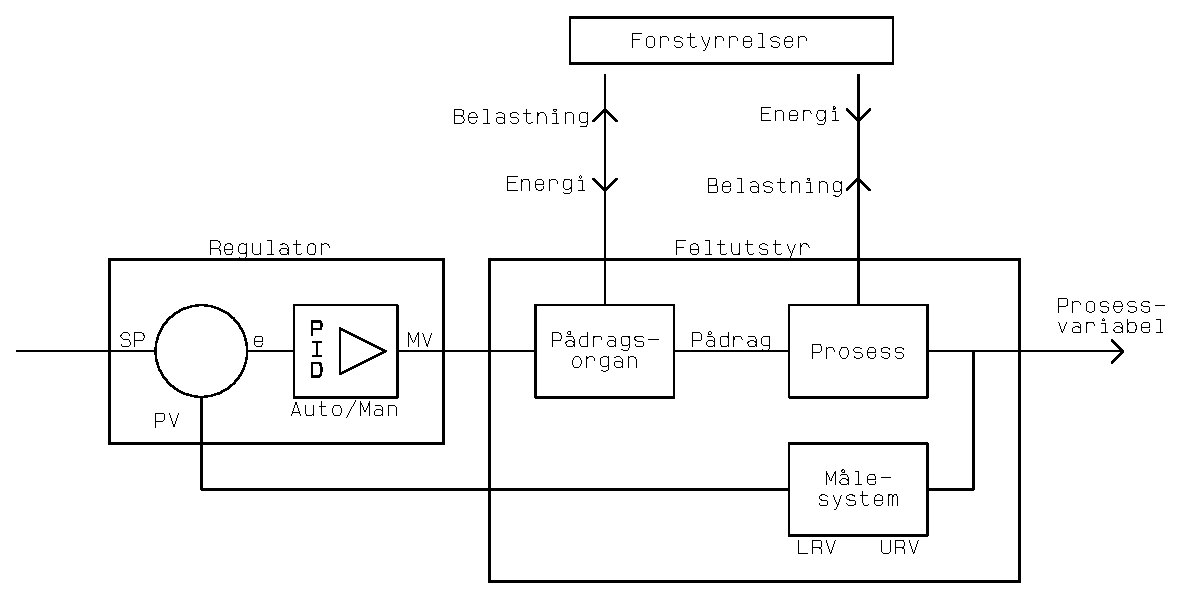
\includegraphics[width=1\textwidth]{./regblock.eps}$$

\vskip 5pt 
Direktevirkende regulator og reverstert regulator

\vskip 5pt 
En reversvirkende regulator er satt opp slik at pådraget øker når
PV er mindre enn SP. $e=SP-PV$

\vskip 5pt 
En direktevirkende regulator er satt opp slik at pådraget øker når
PV er større enn SP. $e=PV-SP$
\vfil \eject
\subsection{Optimalisering}
\subsubsection{Tims rule of tumb}
\begin{enumerate}
	\item Bare jobb med en justering av et parameter om gangen. Når du justerer flere mister du kontrollen. 
	\item Proporsjonalleddet bestemmer hvor fort en prosess går mot settpunktet. Stor proporsjonalforsterkning vil få prosesse til å nå settpunktet raskt, men du vil få et oversving og mest sannsynlig oscillasjoner. Om du setter P-forsterkningen for lavt unngår du oscillasjoner men det vil ta lang tid å nå settpunktet. Start med I-leddet og D-leddet avslått og øk forsterkningen forsiktig  fra 0.25 (0.25, 0.5, 1, 2, 4, 8, 16) til du får oscillasjoner. Reduser så forsterkningen litt. En regulator med bare P-ledd vil ha et statisk avvik fra settpunktet. 
	\item I-leddet virker ved å fjerne feil. Det kan hjelpe til med å redusere oscillasjoner og statiske avvik, men feil justering vil føre til oversving og oscillasjoner. Reduser I-tiden i forsiktig til oscillasjoner og statisk avvik er elliminert. 
	\item D-leddet er ikke nødvendig i de fleste tilfeller om det er akseptabelt med oversving. Om du trenger D-leddet øk forsiktid d-tiden til du er fornød med responsen på variasjoner i prosessen  (SP forandringer).
\end{enumerate}





\subsubsection{Ziegler\_nichols svingemetode}
\begin{enumerate}
\item Regulatoren må stå i manuell modus.
\item Få prosessen til arbidpunktet ved å justere MV manuelt eller ved å bruke en ikke optimalisert regulering. Det er viktig at PV er tilnærmet lik SP da prosessen kan ha andre egenskaper ved andre verdier. 
\item Sett regulatoren til å bare bruke P-leddet. Sett I-ledd til uendelig eller så høyt den går. NB noen regulatorer slår av I-leddet om du setter I-tiden til 0, sjekk  manualen. Sett D-leddet til 0. 
\item Sett regulatoren i automatisk modus.
\item Øk $K_p$ (du kan starte med $K_p$ = 1) inntil det oppstår stående svingninger
i sløyfen etter et sprang i settpunktet. (Reguleringssystemet er da
på stabilitetsgrensen.) Spranget skal være lite, f.eks. 5\% av referansens
verdiområde, slik at prosessen holder seg nokså nær arbeidspunktet.
Men spranget må heller ikke være så lite at responsen ikke kan observeres.
Obs: Pass på at pådraget ikke når sine metningsgrenser (maks, min)
under eksperimentene. Hvis pådraget når en av disse grensene,
vil det kunne bli stående svingninger uansett hvor stor K p vi bruker.
F.eks. kan vi da ha funnet at K pk = 1000000 gir stående svingninger,
og ihht. formelen for K p i en PI-regulator skal da K p settes lik
450000, som temmelig sikkert gir et ustabilt reguleringssystem! Det
gjelder altså å finne den minste K p u som gir stående svingninger
uten at pådraget når metningsgrensene. Dette krever at du overvåker
pådraget under eksperimentene og passer på å ikke ha så store settpunktsendringer
at pådraget når maksimum- eller minimumsverdiene.
\item Noter $K_p$ -verdien som gir stående svingninger. Denne verdien kalles
	den kritiske forsterkning $K_{Pu}$. Noter også perioden $P_u$ for de stående
svingningene. Denne perioden kalles den kritiske perioden.
\item Beregn regulatorparametrene i henhold til tabellen  og legg dem
inn i regulatoren. Forhåpentligvis får da reguleringssystemet tilfredsstillende
ytelse. Er stabiliteten i reguleringssløyfen dårlig (store oversving
i responsene), er det enklest å prøve å redusere $K_p$ .
\end{enumerate}
\begin{tabular}{|c|c|c|c|}
\hline 
 &  &  & \tabularnewline
\hline 
P-regulator & 0.5$K_{pk}$ & $\infty$ & 0\tabularnewline
\hline 
PI-regulator & 0.45$K_{pk}$ & $\frac{P_{u}}{1.2}$ & 0\tabularnewline
\hline 
PID-regulator & 0.6$K_{pk}$ & $\frac{P_{u}}{2}$ & $\frac{P_{u}}{8}=\frac{T_{i}}{4}$\tabularnewline
\hline 
\end{tabular}




\subsubsection{Skogestads metode}

Skogestad har angitt PID-regulatorinnstilling for en rekke ulike prosesstyper. Vi bruker den på følgende prosesstyper:
\begin{itemize}
\item Selvstabiliserende med tidsforsinkelse. (Eksempel på
prosess med slik dynamikk er varmeveksler.)
\item Selvstabiliserende med neglisjerbar tidsforsinkelse. Ved denne type prossess vil Z\&N være vanskelig å få til å svinge
\item Integrerende med tidsforsinkelse 
(Eksempel: Tank med transportbånd, som flistanken.)
\item Integrerende uten tidsforsinkelse (Eksempel: Væsketank styrt av pumpe eller ventil på inn- eller utløp.)
\end{itemize}

\paragraph{Innstilling av PI-regulator for tidkonstant med tidsforsinkelse}

~

\includegraphics{Sprang_selvregulerende.eps}

\[
K_{P}=\dfrac{\tau}{K\left(T_{C}+\theta\right)}
\]

\[
T_{i}=min[\tau,c(T_{c}+\theta]
\]

Her bruker en den minste verdien av $\tau$ og c (c er 2 eller 4)

\includegraphics[width=1\textwidth]{Reg_step_response01}

Her er et eksempel på en prosess med tidsforsinkelse. Når vi leser
av garfen får vi at

\begin{eqnarray*}
\theta & = & 0.5s\\
\tau & = & 5s\\
K & = & 2
\end{eqnarray*}

Det gir oss:
\[
K_{P}=\dfrac{\tau}{K\left(T_{C}+\theta\right)}=\dfrac{5}{2(0.5+0.4)}=2.5
\]

c=2 er her mindre en T=5 som gir 
\[
T_{i}=c(T_{c}+\theta)=2(0.5+0.5)=2
\]

Det gir følgende innregulering på et sprang fra 50 til 55. 

\includegraphics[width=1\textwidth]{Reg_innreg_skogestad01}

\paragraph{Innstilling av PI-regulator for integrator med tidsforsinkelse}

~

\includegraphics{Sprang_integrerendeprosess.eps}

\[
K_{i}=\dfrac{\Delta PV}{\Delta MV\cdot\Delta t}
\]

\[
Kp=\dfrac{1}{K_{i}\left(T_{c}+\theta\right)}
\]

\[
T_{i}=c\left(T_{c}+\theta\right)
\]

Eksempel:

\includegraphics[width=1\textwidth]{Reg_step_integrator}

\[
K_{i}=\dfrac{\Delta PV}{\Delta MV\cdot\Delta t}=\dfrac{40\%}{5\%\cdot8s}=1/s
\]
\[
\tau=0.5s
\]

\[
Kp=\dfrac{1}{K_{i}\left(T_{c}+\theta\right)}=\dfrac{1}{1}
\]

\[
T_{i}=c\left(T_{c}+\theta\right)=2\left(0.5+0.5\right)=2
\]
Som gir følgende innregulering

\includegraphics[width=1\textwidth]{Reg_innreg_skogestad02}
\vfil  \eject


\section{Industriroboter}
Hva er en industi robot?

\vskip 5pt 
Industrial robot as defined by iso 8373:2012:
An automatically controlled, reprogrammable, multipurpose manipulator.
Programmable in three or more axes, which can be either fixed in place or mobile for use in industrial automation applications.

\vskip 5pt 
Klassifiskajson av industriroboter ut fra mekanisk struktur. 
\begin{itemize}[noitemsep]
	\item Linære roboter (Cartesian og Gantry)
	\item SCARA robots
	\item Artikulert robot (den vi har)
	\item Parallelle roboter (delta)
\end{itemize}


Classification by mechanical structure:
Linear robots (including cartesian and gantry robots)
SCARA robots
Articulated robots
Parallel robots (delta)
Cylindrical robots
Others
Not classified
Figures 1.1 illustrates the mechanical c

\vskip 10pt 
Hva kjennetegner en industriell robot:
\begin{itemize}[noitemsep]
\item den kjører automatisk
\item den kan reprogrammeres
\item den har en arm med mer en tre akser som en kan feste ulike verktøy på
\item den kan enten stå fast eller være flyttbare
\item den er laget for å løse industrelle oppgaver 
\end{itemize}

Ulike industrielle roboter kan være:
\begin{itemize}[noitemsep]
\item Linære roboter
\item SCARA roboter
\item Parallelle roboter
\item Artikulerte roboter
\item Sylindriske roboter
\item 
\end{itemize}

\vskip 10pt 
Eksempler på industrielle bruksområder:


\begin{itemize}[noitemsep]
\item Forflytting av metall i deleproduksjon eller støyping
\item palletering
\item sveising
\item lakkering
\item pakking
\item automatisk lagersystem
\end{itemize}
\vfil  \eject
\subsection{Robotstudio}

Installasjon:
\begin{itemize}[noitemsep]
	\item Last ned installasjonsfeil fra fagbibliotek
	\item Installer robotware i fra
	\item Koble opp til lisensserver og hent ut en commuter lisens for 90 dager(max).
\end{itemize}


\section{Utstyr}
\subsection{Gand RIO-trainer}

Kortet kobles til PLS med en USB kabel og en trenger en USB til seriel
driver (CH340). 

\includegraphics[width=1\textwidth]{./GandRioTrainer.jpg}
\small
\begin{tabular}{|c|c|c|c|}
\hline 
\multicolumn{4}{|c|}{Modbus Data Table}\tabularnewline
\hline 
\hline 
IO & Tilkobling & Register & \tabularnewline
\hline 
Encoder &  & 0000H & Enkoder telleverdi\tabularnewline
\hline 
DO1 & åpen kollektor & 0001H & bit0\tabularnewline
\hline 
DO2 & åpen kollektor & 0001H & bit1\tabularnewline
\hline 
DO3 & åpen kollektor & 0001H & bit2\tabularnewline
\hline 
DO4 & åpen kollektor & 0001H & bit3\tabularnewline
\hline 
PWM1 & åpen kollektor & 0002H & AO 0 (PWM)\tabularnewline
\hline 
PWM2 & åpen kollektor & 0003H & AO 1 (PWM)\tabularnewline
\hline 
PWM3 & åpen kollektor & 0004H & AO 2 (PWM)\tabularnewline
\hline 
DI1 & 24VDC & 0005H & bit0\tabularnewline
\hline 
DI2 & 24VDC & 0005H & bit1\tabularnewline
\hline 
DI3 & 24VDC & 0005H & bit2\tabularnewline
\hline 
DI4 & 24VDC & 0005H & bit3\tabularnewline
\hline 
DI5 & 24VDC & 0005H & bit4\tabularnewline
\hline 
DI6 & 24VDC & 0005H & bit5\tabularnewline
\hline 
AI2 & 4-24mA/0-5V & 0006H & AI2\tabularnewline
\hline 
AI1 & 4-24mA/0-5V & 0007H & AI1\tabularnewline
\hline 
\end{tabular}
\normalsize
\vfil \eject
\section{Instrumenter}
\subsection{multimeter}
\subsection{loop claibrator}
\subsection{nettverkstester}
\subsection{megger}
\subsection{kontinuitetstester}







\section{Software}
\subsection{Oversikt}

\small
\begin{tabular}{|l|l|l|l|}
\hline 
\multicolumn{4}{|c|}{Oversikt over installert software}\tabularnewline
\hline 
\hline 
	Program/pakke & link & Hva & Installert\tabularnewline
\hline 
Codesys& &Program &\tabularnewline
\hline 
OSCAT basic& &package &\tabularnewline
\hline 
PFC 200& &package &\tabularnewline
\hline 
RPI& &package &\tabularnewline
\hline 
Gand Bibliotek& &library &\tabularnewline
\hline 
Gand Visustyle& &Visustyle &\tabularnewline
\hline 
Wago 750-354& &devicedescription &\tabularnewline
\hline 
beckhoff ethercat& &devicedescription &\tabularnewline
\hline 
PC|Schematic& &Program &\tabularnewline
\hline 
WinPCap& &driver &\tabularnewline
\hline 
& & &\tabularnewline
\hline 
\end{tabular}
\normalsize
\vfil \eject

\subsection{PcSchematic}
\subsection{Codesys}
\subsection{Codesys}







\section{PLS}
\includegraphics[width=1\textwidth]{./plsutgangsprogram.eps}
\vfil \eject


\section{Formelsamling}

\subsection{Elektroteknikk}
\vskip 2.5pt
\subsubsection*{Ohms lov}
\vskip 2.5pt
$U=R\cdot I$.
\vskip 2.5pt
\subsubsection*{Kirchoffs lover}
\vskip 2.5pt  
Strøm $\Sigma I=0$\\
\vskip 2.5pt  
$I=I_{1}+I_{2}+\cdot\cdot\cdot+I_{n}$\\
\vskip 2.5pt  
$R=\dfrac{1}{\dfrac{1}{R_{1}}+\dfrac{1}{R_{2}}+\cdot\cdot\cdot+\dfrac{1}{R_{n}}}$
\vskip 2pt
 Spenning $\Sigma U=0$\\
\vskip 2.5pt  
$U=U_{1}+U_{2}+\cdot\cdot\cdot+U_{n}$\\
\vskip 2.5pt  
$R=R_{1}+R_{2}+\cdot\cdot\cdot+R_{n}$\\
\vskip 2pt
Lederresistans: $ R=\frac{\rho\cdot l}{A}$ 
\vskip 2pt
Kortsluttningstrøm $I_{k}=\frac{E}{R_{i}+R_{ytre}}$
\vskip 2pt
Elektrisk effekt: $P=\frac{W}{t}$
\vskip 2pt  
Effektloven: $P=U\cdot I\cdot \sqrt{3} \cdot \cos \varphi$
\vskip 2.5pt  
Virkningsgrad: $\eta=\frac{P_{avgitt}}{P_{tilf\\ort}}$
\vskip 2.5pt
Synkron hastihet: $n_1=\frac{2\cdot f}{P}$
\vskip 2.5pt 
Sakking: $S=\frac{n_1-n}{n_1}$
\vskip 2.5pt 
\subsection{Reguleringsteknikk}
\vskip 2.5pt 
\subsubsection*{PID-regulator}
$MV=$\\
$K_p(e+1/TN \int e dt + TV de/dt)+BIAS$\\
\vskip 2.5pt
$Direkte e=PV-SP$\\
$Reverserende e=SP-PV$\\
\subsubsection*{Ziegler \& Nichols svingemetode}
\subsubsection*{P-regulator}
$K_p = 0.5\cdot K_u$
\subsubsection*{PI-regulator}
$K_p = 0.45\cdot K_u$\\
$T_i = 0,83\cdot T_u$\\
\subsubsection*{PID-regulator}
$K_p = 0.6\cdot K_u$\\
$T_i = 0,5\cdot T_u$\\
$T_d = 0,125\cdot T_u$\\
\vskip 2.5pt 
\subsubsection*{Prosessdynamikk}
\vskip 2.5pt 
$\theta$=døtid
\vskip 2.5pt 
$ \text{Tidskonstant finnes når} \Delta PV_{63\%}$
\vskip 2.5pt 
$\tau$=tidskonstand
\vskip 2.5pt 
$T_C$ velges lik $\theta$
\vskip 2.5pt 
\subsubsection*{Selvstabiliserende}
\vskip 2.5pt 
$K=\dfrac{\Delta PV}{\Delta MV} $
\vskip 2.5pt 
$K_p=\dfrac{\tau}{K(T_C+\theta)}$
\vskip 2.5pt 
$T_i=2(T_C+\theta)$
\vskip 2.5pt 
\subsubsection*{Integrerende}
\vskip 2.5pt 
$K_i=\dfrac{\Delta PV}{\Delta MV \cdot {\Delta t}}$
\vskip 2.5pt 
$K_p=\dfrac{1}{K_i(T_C+\theta)}$
\vskip 2.5pt 
$T_i=2(T_C+\theta)$\\
\subsection{Måleteknikk}
\subsubsection*{Kalibrering}
Feilprosent av span:\\
$Error=\frac {IUT-Standard}{Span} \cdot 100\% $\\
\vskip 2.5pt 
Skaleringsformel:
\vskip 2.5pt 
$\dfrac{x-x_{start}}{x_{range}}=\dfrac{y-y_{start}}{y_{range}}$\\
Eksempel: $\dfrac{12mA-4mA}{16mA}=\dfrac{50\%-0\%}{100\%}$
\subsubsection*{Flowmåling}
\vskip 2.5pt 
\vskip 2.5pt 
\vskip 2.5pt 
Reynoldstall: $Re=\dfrac {D \cdot v \cdot \rho}{\mu}$\\
\vskip 2.5pt 
Bernoulli's formel:\\
$z_1 \rho g + {v_1^2 \rho \over 2} + P_1 = z_2 \rho g + {v_2^2 \rho \over 2} + P_2$\\
\vskip 2.5pt 
\subsubsection*{Law of Continuity}
$\rho_1 A_1 \overline{v_1} = \rho_2 A_2 \overline{v_2} = \cdots \rho_n A_n \overline{v_n}$\\
\\
$W = \rho A \overline{v}$\\\\
$Q=A_1 \overline{v_1} = A_2 \overline{v_2}$\\

Massestrøm: $W=\frac{m}{t}$\\
\vskip 2.5pt 
Volumstrøm: $Q=\frac{V}{t}$\\
\vskip 2.5pt 
Massetetthet: $\rho=\frac{m}{V}$\\
\vskip 2.5pt 
\subsubsection*{Trykkbaserte strømningsmålere}
Måleblende: $Q=k\cdot \sqrt{\Delta p}$\\
\vskip 2.5pt 
Måleblende med varierende $\rho$: $Q=k\cdot \sqrt{\frac{\Delta p}{\rho}}$\\
\vskip 2.5pt
Kvadratrot uttrekker:\\
s = signal i prosent (0-1)\\
$s_{ut}=\sqrt{s_{inn}}$\\
\subsubsection*{Hastighetsbaserte strømningsmålere}
Turbin og Vortex:\\
$Q=kf$\\
Elektromagnetisk:\\
$E=Blv$\\
Ultralyd:\\
$Q = k {t_{up} - t_{down} \over (t_{up})(t_{down})}$\\
 
\subsection{Nivåmåling}

$P = \rho \cdot g \cdot h $\\
\subsection{Temperaturmåling}
$R_T = R_{ref}[1 + \alpha(T - T_{ref})]$\\
European $\alpha=0.00385$\\
American $\alpha=0.00392$\\
\vfil \eject


\section{Tabeller}

\begin{center}
	\begin{tabular}{| m{4cm} |m{4cm} |m{4cm} |} 
\hline
	\multicolumn{3}{|c|}{\textbf{\cellcolor[HTML]{D5D5D5}Oversikt over laboppgaver}} \\
\hline
\hline
\rowcolor [HTML]{D5D5D5}
Finn eller beregn 		&Verdi				&Kommentar							\\ \cline{1-3}
Ib - belastningsstrøm		&				&								\\ \cline{1-3}
In – Nominell størrelse vern	&				&$Ib \leq In$							\\ \cline{1-3}
Karakteristikk			&				&								\\ \cline{1-3}
Referanseinstallasjonsmetode	&				&Figur D.1 side 118						\\ \cline{1-3}
2- eller 3-leder		&				&								\\ \cline{1-3}
PVC eller PEX			&				&								\\ \cline{1-3}
Strømføringsevne (Iz) 		&				&Tabell 6 side 81						\\ \cline{1-3}
Tverrsnitt			&				&								\\ \cline{1-3}
Omgivelsestemperatur		&$Temp:\hskip 1cm k_{temp}:$	&Tabell D.1 side 117						\\ \cline{1-3}
Nærføring			&$Antall:\hskip 0.9cm k_{ner}:$		&Tabell D.2 side 119					\\ \cline{1-3}
Ny Strømføringsevne (Iz)	& 				&$I_z\cdot k_{temp} \cdot k_{ner}$ 				\\ \cline{1-3}
Krav 1				&				&$Ib \leq In \leq Iz$						\\ \cline{1-3}
Krav 2				&				&$I2 \leq 1,45 \cdot Iz$					\\ \cline{1-3}
Motstand leder ($R_l$) 		&				&$R_l= \dfrac {\rho \cdot l \cdot \sqrt{3} \cdot cos\phi}{A}$ 	\\ \cline{1-3}
Motstand ved 70°C ($R_{l_{70}}$)	&				&$R_{l_{70}}=R_l \cdot 1,2$				\\ \cline{1-3}
Spenningsfall $\Delta U$	&				&$\Delta U=R_{l_{70}} \cdot I_b$				\\ \cline{1-3}
Spenningsfall \%  		&				&$\Delta U_{i \%}= \dfrac{ \Delta U}{U} \cdot 100\%$		\\ \cline{1-3}
Vurdering spenningsfall 	&				&								\\ \cline{1-3}
Kontroller at vernet ikke slår ut på startstrømmen 	& 	&$I_{start}< I_4$						\\ \cline{1-3}
Ikmin på siste punkt		& 				&								\\ \cline{1-3}
Vernets I5			& 				&								\\ \cline{1-3}
Løser vernet ut momentant ved kortslutning		& 	&$I_5\leq Ik_{min}$ 						\\ \cline{1-3}
Hvor lang tid tar det før vernet løser ut		& 	& 								\\ \cline{1-3}
Kontroller maksimal kabellengde 			&	&Tabell 10 side 102 						\\ \cline{1-3}
Tåler vernet største kortslutning 			& 	&$Ik_{maks} \leq I_{cu}$ 					\\ \cline{1-3}
Hvor lenge tåler kabelen kortslutningen  		& 	&D.4 side 121  $t=(k \cdot \frac{S}{I})^2$ 			\\ \cline{1-3}
Løser sikringen ut før kabelen blir ødelagt? 		& 	&$0,1s < t < 5s$ 						\\ \cline{1-3}


		
\end{tabular}
\end{center}



	
\newpage
\includegraphics[width=1\textwidth]{002.eps}
\vfil \eject
\includegraphics[angle=90,height=1\textheight]{./chemistry12.eps}
\vfil \eject
\includegraphics[width=1\textwidth]{calibrate03.eps}
\includegraphics[width=1\textwidth]{calibrate04.eps}
\includegraphics[width=0.5\textwidth]{current09.eps}
\includegraphics[width=0.5\textwidth]{current10.eps}
\includegraphics[width=0.5\textwidth]{current11.eps}
\includegraphics[width=0.5\textwidth]{current12.eps}
\includegraphics[width=0.5\textwidth]{current13.eps}
\includegraphics[width=0.5\textwidth]{current29.eps}
\includegraphics[width=0.5\textwidth]{current30.eps}
\includegraphics[width=0.5\textwidth]{current31.eps}
\includegraphics[width=1\textwidth]{plc_048.eps}
\includegraphics[width=1\textwidth]{plc_052.eps}
\includegraphics[width=1\textwidth]{pressure76.eps}

\vfil \eject
\end {document}
